% ============================================================
% 第18章 平行四边形 — 人教版八年级下册
% 编译命令：xelatex -interaction=nonstopmode 第18章_平行四边形.tex
% ============================================================
\documentclass[12pt, a4paper]{ctexart}
\usepackage[margin=2.2cm]{geometry}
\usepackage{amsmath, amssymb}
\usepackage{enumitem}
\usepackage{tcolorbox}
\usepackage{booktabs}
\usepackage{array}
\usepackage{fancyhdr}
\usepackage{xcolor}
\usepackage{tikz}
\usepackage{hyperref}
\usepackage{graphicx}
\usepackage{multirow}
\usepackage{pgfplots}
\pgfplotsset{compat=1.18}

% 颜色定义
\definecolor{mainblue}{RGB}{41, 98, 168}
\definecolor{lightblue}{RGB}{230, 240, 255}
\definecolor{tipgreen}{RGB}{34, 139, 87}
\definecolor{lightgreen}{RGB}{235, 250, 240}
\definecolor{warnred}{RGB}{200, 50, 50}
\definecolor{lightred}{RGB}{255, 240, 240}
\definecolor{examorange}{RGB}{210, 120, 20}
\definecolor{lightorange}{RGB}{255, 248, 235}
\definecolor{apppurple}{RGB}{120, 60, 170}
\definecolor{lightpurple}{RGB}{245, 238, 255}

% 页眉页脚
\pagestyle{fancy}
\fancyhf{}
\fancyhead[L]{\small\textcolor{mainblue}{\textbf{人教版八年级下册 · 第18章 平行四边形}}}
\fancyhead[R]{\small\textcolor{mainblue}{家教讲义}}
\fancyfoot[C]{\small —\ \thepage\ —}
\renewcommand{\headrulewidth}{0.6pt}
\renewcommand{\headrule}{\hbox to\headwidth{\color{mainblue}\leaders\hrule height \headrulewidth\hfill}}
\renewcommand{\footrulewidth}{0pt}

% tcolorbox 样式
\newtcolorbox{knowledgebox}[1][]{%
  colback=lightblue, colframe=mainblue,
  fonttitle=\bfseries\large, title=#1,
  arc=3mm, boxrule=0.8pt,
  left=8pt, right=8pt, top=6pt, bottom=6pt
}

\newtcolorbox{tipbox}[1][]{%
  colback=lightgreen, colframe=tipgreen,
  fonttitle=\bfseries, title=#1,
  arc=2mm, boxrule=0.6pt,
  left=6pt, right=6pt, top=4pt, bottom=4pt
}

\newtcolorbox{warnbox}[1][]{%
  colback=lightred, colframe=warnred,
  fonttitle=\bfseries, title=#1,
  arc=2mm, boxrule=0.6pt,
  left=6pt, right=6pt, top=4pt, bottom=4pt
}

\newtcolorbox{examplebox}[1][]{%
  colback=lightorange, colframe=examorange,
  fonttitle=\bfseries, title=#1,
  arc=3mm, boxrule=0.8pt,
  left=8pt, right=8pt, top=6pt, bottom=6pt
}

\newtcolorbox{appbox}[1][]{%
  colback=lightpurple, colframe=apppurple,
  fonttitle=\bfseries, title=#1,
  arc=3mm, boxrule=0.8pt,
  left=8pt, right=8pt, top=6pt, bottom=6pt
}

\setCJKmainfont{Hiragino Sans GB}
\setCJKsansfont{Heiti SC}

\begin{document}

% ============ 标题页 ============
\begin{center}
{\Huge\bfseries\textcolor{mainblue}{第18章\quad 平行四边形}}\\[12pt]
{\Large\textcolor{gray}{家\ 教\ 讲\ 义}}\\[8pt]
\rule{0.6\textwidth}{1pt}\\[8pt]
{\normalsize 适用：人教版\quad 八年级下册\quad |\quad 课时：6课时}
\end{center}
\vspace{10pt}

% ============ 第一部分：知识点讲解 ============
\section*{\textcolor{mainblue}{一、知识点讲解}}

\subsection*{18.1\quad 平行四边形的性质}

\begin{knowledgebox}[平行四边形的定义]
\textbf{平行四边形}：两组对边分别平行的四边形叫做平行四边形。记作 $\square ABCD$。
\end{knowledgebox}

\begin{center}
\begin{tikzpicture}[scale=1.2]
  \coordinate (A) at (0,0);
  \coordinate (B) at (4,0);
  \coordinate (C) at (5.5,2);
  \coordinate (D) at (1.5,2);
  \draw[thick, mainblue] (A) -- node[below]{$a$} (B) -- node[right]{$b$} (C) -- node[above]{$a$} (D) -- node[left]{$b$} (A);
  \draw[thick, dashed, mainblue] (A) -- node[above right, sloped]{$d_1$} (C);
  \draw[thick, dashed, mainblue] (B) -- node[above left, sloped]{$d_2$} (D);
  \node[below left] at (A) {$A$};
  \node[below right] at (B) {$B$};
  \node[above right] at (C) {$C$};
  \node[above left] at (D) {$D$};
  \coordinate (O) at ($(A)!0.5!(C)$);
  \fill (O) circle(1.5pt) node[right]{$O$};
\end{tikzpicture}
\end{center}

\begin{knowledgebox}[平行四边形的性质]
\begin{enumerate}[label=\arabic*.]
  \item \textbf{对边平行且相等}：$AB \parallel CD$，$BC \parallel AD$；$AB = CD$，$BC = AD$。
  \item \textbf{对角相等}：$\angle A = \angle C$，$\angle B = \angle D$。
  \item \textbf{邻角互补}：$\angle A + \angle B = 180°$（相邻两角之和为 $180°$）。
  \item \textbf{对角线互相平分}：$OA = OC$，$OB = OD$。
\end{enumerate}
\end{knowledgebox}

\begin{warnbox}[易错提醒]
\begin{enumerate}[label=\arabic*.]
  \item "对边相等"和"对角相等"中的"对"字不能丢。平行四边形的邻边不一定相等，邻角也不一定相等。
  \item 平行四边形的对角线\textbf{不一定相等}（只有矩形对角线相等）。
  \item 平行四边形的对角线\textbf{不一定垂直}（只有菱形对角线垂直）。
\end{enumerate}
\end{warnbox}

\subsection*{18.2\quad 平行四边形的判定}

\begin{knowledgebox}[平行四边形的判定方法（5种）]
要证明一个四边形是平行四边形，可以用以下任一方法：
\begin{enumerate}[label=\textbf{方法\arabic*：}]
  \item \textbf{两组对边分别平行}（定义法）。\\
  即 $AB \parallel CD$ 且 $AD \parallel BC$。
  \item \textbf{两组对边分别相等}。\\
  即 $AB = CD$ 且 $AD = BC$。
  \item \textbf{一组对边平行且相等}。\\
  即 $AB \parallel CD$ 且 $AB = CD$。
  \item \textbf{两组对角分别相等}。\\
  即 $\angle A = \angle C$ 且 $\angle B = \angle D$。
  \item \textbf{对角线互相平分}。\\
  即 $OA = OC$ 且 $OB = OD$。
\end{enumerate}
\end{knowledgebox}

\begin{tipbox}[判定口诀]
判定平行四边形的方法可以简记为：
\begin{center}
\textbf{两平、两等、一平一等、两对角相等、对角线平分}
\end{center}
其中"一平一等"指"一组对边平行且相等"，这是最常用的方法之一。
\end{tipbox}

\begin{warnbox}[易错提醒]
\begin{enumerate}[label=\arabic*.]
  \item "一组对边平行，另一组对边相等"不能判定平行四边形！（反例：等腰梯形）
  \item "对角线相等"不能判定平行四边形！（反例：等腰梯形）
  \item "对角线互相垂直"不能判定平行四边形！（反例：筝形）
\end{enumerate}
\end{warnbox}

\subsection*{18.3\quad 矩形}

\begin{knowledgebox}[矩形的定义和性质]
\textbf{矩形}：有一个角是直角的平行四边形叫做矩形。

矩形除具有平行四边形的所有性质外，还有以下特殊性质：
\begin{enumerate}[label=\arabic*.]
  \item 四个角都是直角。
  \item \textbf{对角线相等}：$AC = BD$。
  \item 对角线互相平分（来自平行四边形性质）。
\end{enumerate}
\end{knowledgebox}

\begin{knowledgebox}[矩形的判定]
\begin{enumerate}[label=\textbf{方法\arabic*：}]
  \item 有一个角是直角的平行四边形。
  \item 对角线相等的平行四边形。
  \item 三个角是直角的四边形（或四个角都是直角的四边形）。
\end{enumerate}
\end{knowledgebox}

\begin{center}
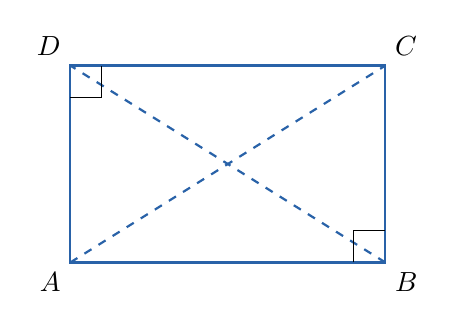
\begin{tikzpicture}[scale=1.0]
  \coordinate (A) at (0,0);
  \coordinate (B) at (4,0);
  \coordinate (C) at (4,2.5);
  \coordinate (D) at (0,2.5);
  \draw[thick, mainblue] (A) -- (B) -- (C) -- (D) -- cycle;
  \draw[thick, dashed, mainblue] (A) -- (C);
  \draw[thick, dashed, mainblue] (B) -- (D);
  \draw (3.6,0) -- (3.6,0.4) -- (4,0.4);
  \draw (0,2.1) -- (0.4,2.1) -- (0.4,2.5);
  \node[below left] at (A) {$A$};
  \node[below right] at (B) {$B$};
  \node[above right] at (C) {$C$};
  \node[above left] at (D) {$D$};
\end{tikzpicture}
\end{center}

\subsection*{18.4\quad 菱形}

\begin{knowledgebox}[菱形的定义和性质]
\textbf{菱形}：有一组邻边相等的平行四边形叫做菱形。

菱形除具有平行四边形的所有性质外，还有以下特殊性质：
\begin{enumerate}[label=\arabic*.]
  \item \textbf{四条边都相等}。
  \item \textbf{对角线互相垂直}：$AC \perp BD$。
  \item 对角线互相平分（来自平行四边形性质）。
  \item 对角线平分每组对角（每条对角线平分两个对角）。
\end{enumerate}
\end{knowledgebox}

\begin{knowledgebox}[菱形的判定]
\begin{enumerate}[label=\textbf{方法\arabic*：}]
  \item 有一组邻边相等的平行四边形。
  \item 对角线互相垂直的平行四边形。
  \item 四条边都相等的四边形。
\end{enumerate}
\end{knowledgebox}

\begin{center}
\begin{tikzpicture}[scale=1.0]
  \coordinate (A) at (0,0);
  \coordinate (B) at (3,0);
  \coordinate (C) at (4.5,2.5);
  \coordinate (D) at (1.5,2.5);
  \draw[thick, mainblue] (A) -- node[below]{$a$} (B) -- node[right]{$a$} (C) -- node[above]{$a$} (D) -- node[left]{$a$} (A);
  \draw[thick, dashed, mainblue] (A) -- (C);
  \draw[thick, dashed, mainblue] (B) -- (D);
  \coordinate (O) at ($(A)!0.5!(C)$);
  \fill (O) circle(1.5pt) node[below right]{$O$};
  \draw (2.65, 0.85) -- (3.0, 1.05) -- (2.8, 1.4);
  \node[below left] at (A) {$A$};
  \node[below right] at (B) {$B$};
  \node[above right] at (C) {$C$};
  \node[above left] at (D) {$D$};
\end{tikzpicture}
\end{center}

\subsection*{18.5\quad 正方形}

\begin{knowledgebox}[正方形的定义和性质]
\textbf{正方形}：既是矩形又是菱形的四边形叫做正方形。

正方形兼具矩形和菱形的所有性质：
\begin{enumerate}[label=\arabic*.]
  \item \textbf{四条边都相等}。
  \item \textbf{四个角都是直角}。
  \item \textbf{对角线相等、互相垂直、互相平分}。
  \item 对角线平分每组对角。
\end{enumerate}
\end{knowledgebox}

\begin{knowledgebox}[正方形的判定]
\begin{enumerate}[label=\textbf{方法\arabic*：}]
  \item 有一个角是直角的菱形。
  \item 有一组邻边相等的矩形。
  \item 对角线相等且互相垂直的四边形（不必先证平行四边形）。
\end{enumerate}
\end{knowledgebox}

\begin{center}
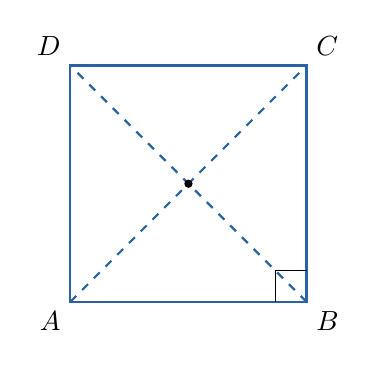
\begin{tikzpicture}[scale=1.0]
  \coordinate (A) at (0,0);
  \coordinate (B) at (3,0);
  \coordinate (C) at (3,3);
  \coordinate (D) at (0,3);
  \draw[thick, mainblue] (A) -- (B) -- (C) -- (D) -- cycle;
  \draw[thick, dashed, mainblue] (A) -- (C);
  \draw[thick, dashed, mainblue] (B) -- (D);
  \draw (2.6,0) -- (2.6,0.4) -- (3,0.4);
  \coordinate (O) at (1.5,1.5);
  \fill (O) circle(1.5pt);
  \node[below left] at (A) {$A$};
  \node[below right] at (B) {$B$};
  \node[above right] at (C) {$C$};
  \node[above left] at (D) {$D$};
\end{tikzpicture}
\end{center}

\subsection*{18.6\quad 四种四边形的关系}

\begin{knowledgebox}[四边形的包含关系]
\begin{center}
\begin{tikzpicture}[scale=0.9]
  % 正方形（最内层）
  \draw[thick, mainblue, fill=lightblue] (0,0) rectangle (4,2.5);
  \node at (2, 1.25) {\textbf{正方形}};
  % 矩形
  \draw[thick, tipgreen] (-0.5,-0.4) rectangle (4.5,2.9);
  \node at (2, 2.9) [above] {\textcolor{tipgreen}{\textbf{矩形}}};
  % 菱形
  \draw[thick, examorange] (-0.5,-0.4) rectangle (4.5,2.9);
  \node at (4.5, 1.25) [right] {\textcolor{examorange}{\textbf{菱形}}};
  % 平行四边形（最外层）
  \draw[thick, warnred] (-1,-0.8) rectangle (5,3.3);
  \node at (2, 3.3) [above] {\textcolor{warnred}{\textbf{平行四边形}}};
\end{tikzpicture}
\end{center}

\textbf{关系总结}：
\begin{itemize}
  \item 正方形 $\subset$ 矩形 $\subset$ 平行四边形
  \item 正方形 $\subset$ 菱形 $\subset$ 平行四边形
  \item 矩形与菱形的交集 $=$ 正方形
\end{itemize}
\end{knowledgebox}

\subsection*{18.7\quad 三角形中位线定理}

\begin{knowledgebox}[三角形中位线定理]
连接三角形两边中点的线段叫做三角形的\textbf{中位线}。

\textbf{定理}：三角形的中位线\textbf{平行于第三边}，且等于第三边的\textbf{一半}。

即：在 $\triangle ABC$ 中，$D$、$E$ 分别是 $AB$、$AC$ 的中点，则
\[
DE \parallel BC, \quad DE = \frac{1}{2}BC
\]
\end{knowledgebox}

\begin{center}
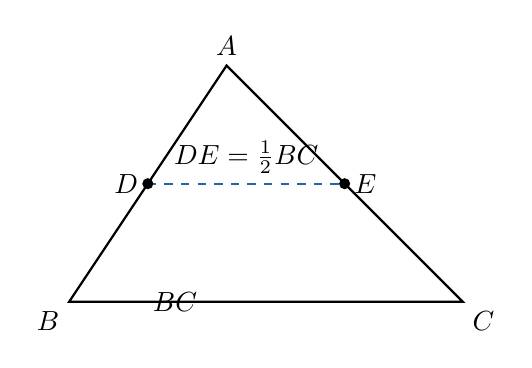
\begin{tikzpicture}[scale=1.0]
  \coordinate (A) at (2,3);
  \coordinate (B) at (0,0);
  \coordinate (C) at (5,0);
  \coordinate (D) at (1,1.5);
  \coordinate (E) at (3.5,1.5);
  \draw[thick] (A) -- (B) -- (C) -- cycle;
  \draw[thick, mainblue, dashed] (D) -- (E);
  \fill (D) circle(2pt) node[left]{$D$};
  \fill (E) circle(2pt) node[right]{$E$};
  \node[above] at (A) {$A$};
  \node[below left] at (B) {$B$};
  \node[below right] at (C) {$C$};
  \node[left] at (1.75,0) {$BC$};
  \node[above] at (2.25,1.5) {$DE=\frac{1}{2}BC$};
\end{tikzpicture}
\end{center}

\begin{tipbox}[中位线定理的应用]
\begin{enumerate}[label=\arabic*.]
  \item 中位线定理常用于证明线段之间的倍分关系和平行关系。
  \item 证明中位线定理的方法：连接 $DE$ 后延长到 $F$，使 $EF = DE$，利用对角线互相平分构造平行四边形。
  \item 三角形有三条中位线，它们构成的中位线三角形面积是原三角形面积的 $\frac{1}{4}$。
\end{enumerate}
\end{tipbox}

% ============ 第二部分：例题精讲 ============
\section*{\textcolor{examorange}{二、例题精讲}}

\begin{examplebox}[【例题1】基础计算——利用平行四边形性质求角]
在平行四边形 $ABCD$ 中，$\angle A = 70°$，求 $\angle B$、$\angle C$、$\angle D$ 的度数。
\end{examplebox}

\textbf{解：}

在平行四边形中：
\begin{itemize}
  \item 邻角互补：$\angle B = 180° - \angle A = 180° - 70° = 110°$。
  \item 对角相等：$\angle C = \angle A = 70°$，$\angle D = \angle B = 110°$。
\end{itemize}

所以 $\angle B = 110°$，$\angle C = 70°$，$\angle D = 110°$。

\begin{tipbox}[方法总结]
平行四边形的角度问题只需牢记两条规则：对角相等、邻角互补。知道一个角，其余三个角都能求出。
\end{tipbox}

\vspace{6pt}

\begin{examplebox}[【例题2】基础计算——利用对角线互相平分]
在平行四边形 $ABCD$ 中，对角线 $AC$ 和 $BD$ 相交于点 $O$，$AC = 10$，$BD = 14$。\\
设 $\triangle OAB$ 的周长为 $L$，$AB = 6$，求 $L$。
\end{examplebox}

\textbf{解：}

平行四边形对角线互相平分：
\[
OA = \frac{AC}{2} = 5, \quad OB = \frac{BD}{2} = 7
\]

$\triangle OAB$ 的周长：
\[
L = OA + OB + AB = 5 + 7 + 6 = 18
\]

\begin{tipbox}[方法总结]
平行四边形对角线互相平分，所以对角线的一半就是从交点到各顶点的线段长。这类问题常与三角形周长或三角形全等结合考查。
\end{tipbox}

\vspace{6pt}

\begin{examplebox}[【例题3】证明题——证明四边形是平行四边形]
\textbf{已知}：四边形 $ABCD$ 中，$AB = CD$，$AD = BC$。\\
\textbf{求证}：四边形 $ABCD$ 是平行四边形。

\begin{center}
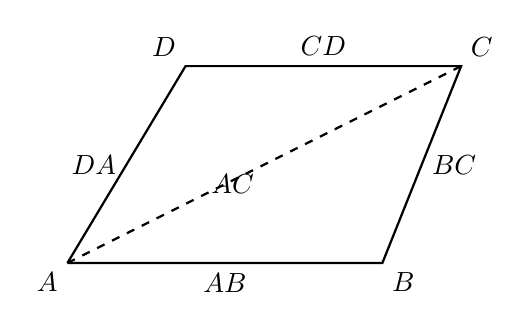
\begin{tikzpicture}[scale=1.0]
  \coordinate (A) at (0,0);
  \coordinate (B) at (4,0);
  \coordinate (C) at (5,2.5);
  \coordinate (D) at (1.5,2.5);
  \draw[thick] (A) -- node[below]{$AB$} (B) -- node[right]{$BC$} (C) -- node[above]{$CD$} (D) -- node[left]{$DA$} (A);
  \draw[thick, dashed] (A) -- node[below left]{$AC$} (C);
  \node[below left] at (A) {$A$};
  \node[below right] at (B) {$B$};
  \node[above right] at (C) {$C$};
  \node[above left] at (D) {$D$};
\end{tikzpicture}
\end{center}
\end{examplebox}

\textbf{证明}：

连接 $AC$。

在 $\triangle ABC$ 和 $\triangle CDA$ 中：
\begin{align*}
AB &= CD \quad \text{（已知）}\\
BC &= DA \quad \text{（已知）}\\
AC &= CA \quad \text{（公共边）}
\end{align*}

$\therefore \triangle ABC \cong \triangle CDA$（SSS）

$\therefore \angle BAC = \angle DCA$（全等三角形对应角相等）

$\therefore AB \parallel CD$（内错角相等，两直线平行）

同理可证 $\angle ACB = \angle CAD$，从而 $AD \parallel BC$。

$\therefore$ 四边形 $ABCD$ 是平行四边形（两组对边分别平行）。\qed

\begin{tipbox}[方法总结]
证明平行四边形时，"两组对边分别相等"常通过连接对角线，证全等三角形来得到平行关系或相等关系。连接对角线是最常用的辅助线。
\end{tipbox}

\vspace{6pt}

\begin{examplebox}[【例题4】易错辨析——条件辨析题]
判断下列命题是否正确，并说明理由：
\begin{enumerate}[label=(\arabic*)]
  \item 一组对边平行，另一组对边相等的四边形是平行四边形。
  \item 对角线相等的四边形是平行四边形。
  \item 对角线互相垂直的四边形是平行四边形。
  \item 一组对边平行且一组对角相等的四边形是平行四边形。
\end{enumerate}
\end{examplebox}

\textbf{解：}
\begin{enumerate}[label=(\arabic*)]
  \item \textbf{错误}。反例：等腰梯形（一组对边平行，另一组对边相等，但不是平行四边形）。
  \item \textbf{错误}。反例：等腰梯形的对角线相等，但它不是平行四边形。
  \item \textbf{错误}。反例：筝形（对角线互相垂直，但不是平行四边形）。
  \item \textbf{正确}。证明：设四边形 $ABCD$ 中 $AB \parallel CD$，$\angle A = \angle C$。\\
  因为 $AB \parallel CD$，所以 $\angle A + \angle D = 180°$（同旁内角互补）。\\
  又 $\angle A = \angle C$，所以 $\angle C + \angle D = 180°$，从而 $AD \parallel BC$。\\
  两组对边分别平行，所以是平行四边形。
\end{enumerate}

\begin{tipbox}[方法总结]
判定平行四边形的条件必须严格满足五种判定方法之一。"一组对边平行，另一组对边相等"不能判定，"对角线相等"不能判定，"对角线互相垂直"也不能判定。要记住这三个易错点。
\end{tipbox}

\vspace{6pt}

\begin{examplebox}[【例题5】综合提高——矩形的判定与性质]
\textbf{已知}：在平行四边形 $ABCD$ 中，对角线 $AC = BD$。\\
\textbf{求证}：平行四边形 $ABCD$ 是矩形。

\begin{center}
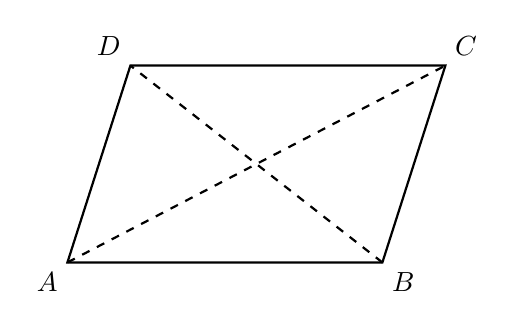
\begin{tikzpicture}[scale=1.0]
  \coordinate (A) at (0,0);
  \coordinate (B) at (4,0);
  \coordinate (C) at (4.8,2.5);
  \coordinate (D) at (0.8,2.5);
  \draw[thick] (A) -- (B) -- (C) -- (D) -- cycle;
  \draw[thick, dashed] (A) -- (C);
  \draw[thick, dashed] (B) -- (D);
  \node[below left] at (A) {$A$};
  \node[below right] at (B) {$B$};
  \node[above right] at (C) {$C$};
  \node[above left] at (D) {$D$};
\end{tikzpicture}
\end{center}
\end{examplebox}

\textbf{证明}：

在 $\triangle ABC$ 和 $\triangle BAD$ 中：
\begin{align*}
AB &= BA \quad \text{（公共边）}\\
BC &= AD \quad \text{（平行四边形对边相等）}\\
AC &= BD \quad \text{（已知）}
\end{align*}

$\therefore \triangle ABC \cong \triangle BAD$（SSS）

$\therefore \angle ABC = \angle BAD$（全等三角形对应角相等）

在平行四边形 $ABCD$ 中，$\angle ABC + \angle BAD = 180°$（邻角互补）。

$\therefore 2\angle ABC = 180°$，$\angle ABC = 90°$。

$\therefore$ 平行四边形 $ABCD$ 是矩形（有一个角是直角的平行四边形）。\qed

\begin{tipbox}[方法总结]
证明一个平行四边形是矩形，只需再证一个角是直角或对角线相等。这里是先用 SSS 全等得到对应角相等，再结合邻角互补求出直角。
\end{tipbox}

\vspace{6pt}

\begin{examplebox}[【例题6】综合题——菱形与勾股定理结合]
在菱形 $ABCD$ 中，对角线 $AC = 8$，$BD = 6$。求：
\begin{enumerate}[label=(\arabic*)]
  \item 菱形的边长。
  \item 菱形的面积。
\end{enumerate}
\end{examplebox}

\textbf{解：}

菱形对角线互相垂直平分。设对角线交点为 $O$，则
\[
OA = \frac{AC}{2} = 4, \quad OB = \frac{BD}{2} = 3, \quad OA \perp OB
\]

\begin{enumerate}[label=(\arabic*)]
  \item 在直角三角形 $AOB$ 中，由勾股定理：
  \[
  AB = \sqrt{OA^2 + OB^2} = \sqrt{16 + 9} = \sqrt{25} = 5
  \]
  菱形的边长为 $5$。

  \item 菱形面积 $= \frac{1}{2} \times d_1 \times d_2 = \frac{1}{2} \times 8 \times 6 = 24$。
\end{enumerate}

\begin{tipbox}[方法总结]
菱形的对角线互相垂直，所以对角线的一半和边长构成直角三角形，可用勾股定理求边长。菱形面积 $= \frac{1}{2} d_1 d_2$，这是菱形特有的面积公式。
\end{tipbox}

\vspace{6pt}

\begin{examplebox}[【例题7】综合题——中位线定理的应用]
在 $\triangle ABC$ 中，$D$、$E$、$F$ 分别是 $BC$、$AC$、$AB$ 的中点。已知 $\triangle ABC$ 的周长为 $24$。
\begin{enumerate}[label=(\arabic*)]
  \item 求 $\triangle DEF$ 的周长。
  \item 若 $\triangle ABC$ 的面积为 $S$，求 $\triangle DEF$ 的面积。
\end{enumerate}
\end{examplebox}

\textbf{解：}
\begin{enumerate}[label=(\arabic*)]
  \item 由三角形中位线定理：
  \[
  DE = \frac{1}{2}AB, \quad EF = \frac{1}{2}BC, \quad DF = \frac{1}{2}AC
  \]
  $\triangle DEF$ 的周长：
  \[
  DE + EF + DF = \frac{1}{2}(AB + BC + AC) = \frac{1}{2} \times 24 = 12
  \]

  \item 由中位线定理，$\triangle DEF$ 的各边分别是 $\triangle ABC$ 对应边的一半。\\
  由于 $\triangle DEF \sim \triangle ABC$，相似比为 $1:2$，面积比为 $1:4$。
  \[
  S_{\triangle DEF} = \frac{1}{4}S
  \]
\end{enumerate}

\begin{tipbox}[方法总结]
三角形中位线定理的核心结论：中位线平行于第三边且等于其一半。三条中位线将原三角形分成四个全等的小三角形，每个面积是原三角形的 $\frac{1}{4}$。
\end{tipbox}

\vspace{6pt}

\begin{examplebox}[【例题8】综合题——平行四边形与全等三角形]
在 $\square ABCD$ 中，$E$、$F$ 分别在 $AD$、$BC$ 上，且 $AE = CF$。\\
\textbf{求证}：$BE = DF$。

\begin{center}
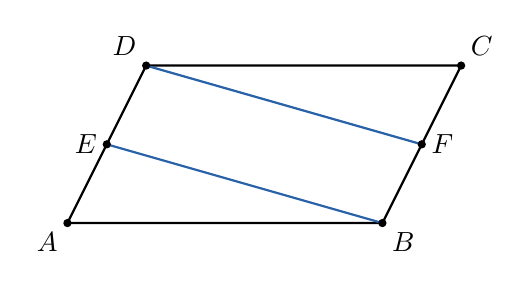
\begin{tikzpicture}[scale=1.0]
  \coordinate (A) at (0,0);
  \coordinate (B) at (4,0);
  \coordinate (C) at (5,2);
  \coordinate (D) at (1,2);
  \coordinate (E) at (0.5,1);
  \coordinate (F) at (4.5,1);
  \draw[thick] (A) -- (B) -- (C) -- (D) -- cycle;
  \draw[thick, mainblue] (E) -- (B);
  \draw[thick, mainblue] (D) -- (F);
  \fill (A) circle(1.5pt) node[below left]{$A$};
  \fill (B) circle(1.5pt) node[below right]{$B$};
  \fill (C) circle(1.5pt) node[above right]{$C$};
  \fill (D) circle(1.5pt) node[above left]{$D$};
  \fill (E) circle(1.5pt) node[left]{$E$};
  \fill (F) circle(1.5pt) node[right]{$F$};
\end{tikzpicture}
\end{center}
\end{examplebox}

\textbf{证明}：

$\because$ 四边形 $ABCD$ 是平行四边形

$\therefore AB \parallel CD$，$AB = CD$（平行四边形对边平行且相等）

$\because$ $E$ 在 $AD$ 上，$F$ 在 $BC$ 上，且 $AE = CF$

$\therefore AD - AE = BC - CF$，即 $ED = BF$

又 $\because AB \parallel CD$，$\therefore AB \parallel ED$

$\therefore$ 四边形 $BEDF$ 是平行四边形（一组对边平行且相等：$AB \parallel ED$ 且 $AB = CD = ED + \ldots$）

让我重新用更直接的方法。

\textbf{证明}：

$\because$ 四边形 $ABCD$ 是平行四边形

$\therefore AB = CD$，$\angle A = \angle C$（平行四边形对边相等，对角相等）

在 $\triangle ABE$ 和 $\triangle CDF$ 中：
\begin{align*}
AB &= CD\\
\angle A &= \angle C\\
AE &= CF
\end{align*}

$\therefore \triangle ABE \cong \triangle CDF$（SAS）

$\therefore BE = DF$（全等三角形对应边相等）。\qed

\begin{tipbox}[方法总结]
在平行四边形中证明线段相等，常用策略是利用平行四边形的性质（对边相等、对角相等）构造全等三角形的条件（SAS、ASA、AAS、SSS），从而得到对应边或对应角相等。
\end{tipbox}

% ============ 第三部分：应用题 ============
\section*{\textcolor{apppurple}{三、应用题}}

\begin{appbox}[【应用1】平行四边形的实际应用——花坛设计]
学校要在一块平行四边形空地上建花坛。已知空地相邻两边长分别为 $20$ 米和 $15$ 米，其中一条边上的高为 $12$ 米。求这块空地的面积。
\end{appbox}

\textbf{解：}

平行四边形的面积 $=$ 底 $\times$ 高。

设 $12$ 米的高对应底边为 $a$ 米。

若底边 $a = 20$ 米，则 $S = 20 \times 12 = 240$ 平方米。

若底边 $a = 15$ 米，则 $S = 15 \times 12 = 180$ 平方米。

需要判断 $12$ 米对应的高是哪条底边。

若高 $12$ 对应底边 $15$，则另一条底边 $20$ 对应的高 $= \frac{180}{20} = 9 < 15$，合理。\\
若高 $12$ 对应底边 $20$，则另一条底边 $15$ 对应的高 $= \frac{240}{15} = 16 > 15$，这意味着高大于邻边，不合理（高不可能大于邻边）。

所以 $12$ 米的高对应的底边是 $15$ 米，空地面积 $= \boxed{180}$ \textbf{平方米}。

\vspace{6pt}

\begin{appbox}[【应用2】中位线的实际应用——测量河宽]
小华要测量一条河的宽度。他先在河的一岸选点 $A$，再在对岸选点 $B$，然后在 $AB$ 同侧选点 $C$（$C$ 不在 $AB$ 上），取 $AC$ 的中点 $D$ 和 $BC$ 的中点 $E$，测得 $DE = 35$ 米。根据三角形中位线定理，河宽 $AB$ 是多少？
\end{appbox}

\textbf{解：}

$D$ 是 $AC$ 的中点，$E$ 是 $BC$ 的中点，$\therefore$ $DE$ 是 $\triangle ABC$ 的中位线。

由中位线定理：
\[
DE = \frac{1}{2}AB
\]
\[
AB = 2 \times DE = 2 \times 35 = \boxed{70} \text{（米）}
\]

河宽为 $70$ 米。

\vspace{6pt}

\begin{appbox}[【应用3】矩形的实际应用——相框制作]
小明要用木条制作一个矩形相框，要求相框的对角线长为 $25$ cm，且长与宽之比为 $3:4$。求相框的长和宽各是多少。
\end{appbox}

\textbf{解：}

设长为 $4x$ cm，宽为 $3x$ cm。

矩形的对角线、长、宽构成直角三角形，由勾股定理：
\[
(4x)^2 + (3x)^2 = 25^2
\]
\[
16x^2 + 9x^2 = 625
\]
\[
25x^2 = 625 \implies x^2 = 25 \implies x = 5
\]

长 $= 4 \times 5 = 20$ cm，宽 $= 3 \times 5 = 15$ cm。

\begin{tipbox}[实际问题建模]
将实际问题转化为数学模型是关键。相框是矩形，对角线已知，长宽比已知，设比例系数列勾股定理方程即可求解。比例设参法是常用技巧。
\end{tipbox}

% ============ 第四部分：课堂练习 ============
\section*{\textcolor{tipgreen}{四、课堂练习}}

\begin{enumerate}
  \item 在平行四边形 $ABCD$ 中，$\angle A - \angle B = 40°$，求 $\angle A$、$\angle B$、$\angle C$、$\angle D$ 的度数。

  \item 在平行四边形 $ABCD$ 中，对角线 $AC$ 和 $BD$ 相交于 $O$，$AC = 16$，$BD = 12$，$AB = 10$。求 $\triangle OAB$ 的周长。

  \item 已知菱形的两条对角线分别为 $6$ 和 $8$，求菱形的面积和边长。

  \item 在矩形 $ABCD$ 中，$AB = 6$，$BC = 8$，$E$ 是 $CD$ 的中点，求 $AE$ 的长。

  \item 如图，在 $\triangle ABC$ 中，$D$、$E$、$F$ 分别是 $AB$、$BC$、$CA$ 的中点。若 $\triangle DEF$ 的周长为 $16$，求 $\triangle ABC$ 的周长。
\end{enumerate}

\vspace{10pt}

\begin{knowledgebox}[参考答案]
\textbf{1.} 由 $\angle A + \angle B = 180°$（邻角互补）和 $\angle A - \angle B = 40°$，\\
联立解得 $\angle A = 110°$，$\angle B = 70°$。\\
由对角相等：$\angle C = \angle A = 110°$，$\angle D = \angle B = 70°$。

\vspace{4pt}
\textbf{2.} $OA = \frac{AC}{2} = 8$，$OB = \frac{BD}{2} = 6$。\\
$\triangle OAB$ 的周长 $= OA + OB + AB = 8 + 6 + 10 = 24$。

\vspace{4pt}
\textbf{3.} 面积 $= \frac{1}{2} \times 6 \times 8 = 24$。\\
对角线互相垂直平分，$OA = 3$，$OB = 4$，边长 $= \sqrt{9+16} = 5$。

\vspace{4pt}
\textbf{4.} $DE = \frac{1}{2}BC = 4$。在 $\triangle ADE$ 中，$AD = BC = 8$，$\angle D = 90°$。\\
$AE = \sqrt{AD^2 + DE^2} = \sqrt{64 + 16} = \sqrt{80} = 4\sqrt{5}$。

\vspace{4pt}
\textbf{5.} $\triangle DEF$ 的各边分别是 $\triangle ABC$ 对应边的中位线，即各边为原边的一半。\\
$\triangle ABC$ 的周长 $= 2 \times 16 = 32$。
\end{knowledgebox}

\vfill
\begin{center}
\small\textcolor{gray}{本讲义仅供教学参考，例题可根据学生水平调整难度。}
\end{center}

\end{document}
